
%This file contains all the details of agent design using files in initialAgentDesign folder




\section{Prefatory Agent Design}\label{subsection:intial_agent_design}
\note{addressed some of these simultaneously (i.e. once I had decided model-based agent, then had to answer question of what model will look like)}
\note{probably best to list these individually with some corresponding discussion}

This section begins by describing four critical parts of the agent design, collectively referred to as the agent's \textit{task environment}: the Actuators, Sensors, Environment, and Performance Element. Further discussion on specific aspects of how the agent function was implemented is then given.
%where the larger multi-faceted problem is broken down into smaller individual sub-problems. 

\subsection{Agent Environment}
\note{Use of italics may not be necessary here}
\note{Should refer to previous works more here}
Here, we refer to conventional terms used to describe agent environments, described in \cite[p.~41]{AIAMA}. The agent's environment is \textit{partially observable}, since it is assumed that it cannot directly observe the location of the target, but must instead use partial information related to the location of the target from noisy sensors. The outcomes of the agent's actions are assumed to be \textit{deterministic}, meaning that if an agent chooses to move to a location, it is assumed to do so without any chance of it accidentally moving to an alternative location. The environment is \textit{sequential}, arising from the fact that future decisions on where the agent should take a sensor reading are influenced by previous locations at which a sensor reading has been taken. The agent is assumed to operate in a 2-dimensional environment, consisting of discrete uniformly spaced grid cells overlaid onto a physical region of space.
%The environment state can then defined by the tuples of the unknown location of the target with the search status.
The unknown location of the target can be described by the set
\[\{x_1, x_2, ..., x_n, x_{n+1}\}\]
where $x_i$ represents the target location being at grid cell $i$ for $i \in \{1, 2, .., n\}$, and $x_{n+1}$ represents that the target is not present. The search status can be described by 
\[ \{ongoing, terminated\_x_1, terminated\_x_2, ..., terminated\_x_n, terminated\_x_{n+1}\} \]
where $ongoing$ represents that the search is continuing and $terminated\_x_i$ is an absorbing terminal state that arises from the agent taking a terminal action indicating the target location, explained further in the subsequent paragraph. It is necessary to include the terminal states in the environment representation in order to specify a \textit{performance measure} for the agent. 
%For technical reasons, the agent's location was also included in the environment state.
The Cartesian product of these sets defines the environment state. For example, the environment might start in state $<x_3, ongoing>$, which represents that a target is located at grid cell 3 and the search is ongoing. $<x_3, terminated\_x_5$ represents that the search has terminated with the agent concluding the target is present at grid cell 5, with the target actually present at grid cell 3. The graphical model shown in Figure \ref{fig:FirstDBNUsed} depicts the conditional independence assumptions made between the hidden state variables, which is explained in Section \ref{subsec:stochasticEnvModel}.
%\note{Goal state not explicitly mentioned - might be worth explicitly stating.}

\subsubsection{Actuators and Sensors}
Here we consider the actions that may be chosen to be performed by actuators and percepts that may be received by sensors. The problem of \textit{target localization} in the context of this chapter requires the agent to move around a discrete grid and use a calibrated sensor to record noisy readings that indicate whether the target is present or not at the location of the reading. It is therefore intuitive to describe the set of possible actions to be performed by the actuators by the set of all $n$ possible grid locations that the agent can move to and take a sensor reading at, indexed by an arbitrary ordering: $\{move\_x_1, move\_x_2, ..., move\_x_n\}$. We add additional actions to this set, $\{terminate\_search\_x_{i}\}$, for $i \in \{1, 2, ..., n, n+1\}$, which lead to an absorbing terminal state representing the agent's conclusion regarding whether a target is present or not, $terminated\_x_{i}$ . The set of percepts that the agent will receive from its sensors come from the binary set \{1, 0\}, indicating the target has or has not been detected, respectively.

\subsection{Performance Measure}\label{sssection:PerfMeas}
The agent's performance measure maps sequences of environment states to the real numbers. Given the above definitions, we decided that environment states of the form
\[ <x_i, terminated\_x_i> \]
should be of high value, as they indicate that the agent has correctly identified the location of the target in the environment. Secondary to this, sequences of environment states that take longer to end in a terminal state should be valued lower than shorter ones, reflecting our desire for the agent to terminate its search in the minimum possible amount of time. Therefore, the performance measure primarily gives high values to the agent when it correctly identifies the location of the target or correctly concludes that the target is not present, with a secondary ordering on value determined by the time taken to come to a conclusion. The actual value of the function only needs to adhere to this ordering, but arbitrarily defined it as:
%\note{Be careful that this agrees with the rest}
\[
Performance Measure(state_1,..., state_t) = 
\begin{cases}
\frac{1}{t} \quad \text{ if } state_t \text{ = } <x_i, terminated\_x_i>
%agent returns correct target location.} 
\\
-1 \quad \text { otherwise. }
\end{cases}
\]

%\[
%Performance Measure(state_1,..., state_t) = 
%\begin{cases}
%\frac{1}{t} \quad \text{ if } state_t \text{ = } <x_i, TERMINATED\_x_i>
%agent returns correct target location.} 
%\\
%\frac{1}{t} \quad \text{ if agent correctly returns target is not present.}
%\\
%-1 \quad \text { if agent returns incorrect target location.}
%\\
%-1 \quad \text{if agent incorrectly returns target is not present}
%\end{cases}
%\]

%The performance measure is assumed to ignore subsequent terminal states. 
It is worth noting that this performance measure provides goal states for the agent:
\[ <x_i, terminated\_x_i> \]



\subsection{Stochastic Environment Model}
\workinprogress
Model-based agents require a concrete implementation of a model of their world, in order to maintain their internal state. The agent's internal state can be thought of as its opinion of what state the world might be in, and its model describes how it believes the world changes over time. Chapter \ref{chapter:Background} outlines the background behind potential models of the stochastic world, including both how internal state can be represented and how internal state can be updated.\par
Hidden Markov Models and Dynamic Bayesian Networks were identified as highly suitable models, due to the fact that they provide a succinct and flexible representation of hidden stochastic world state, as well as efficient online state estimation updating algorithms. We chose to use a Dynamic Bayesian Network (DBN), due to the fact that it can help overcome some of the limitations that HMMs potentially may present (outlined in chapter \ref{chapter:Background}). DBNs also facilitate the incorporation of extra variables with arbitrary conditional dependence relations. This was desirable, since we planned to extend the model to include extra variables, such as battery level, once a basic implementation was shown to work as intended.

The 2-Time Slice DBN used is shown in figure \ref{fig:FirstDBNUsed} describes the agent's world model. A first-order Markov assumption is made, where the current state only depends on the state directly preceding it. Grey coloured variables are \textit{hidden state variables} and are assumed to not be directly observable. Green coloured variables are \textit{control actions} taken by the agent (which use the agent's estimated state) and the peach coloured variables are \textit{evidence variables}, which are assumed to be observable and depend on the hidden world state. 
%The agent's location and the search status hidden state variables are mainly included for technical reasons
\note{maybe re-position figure so text wraps}
\begin{figure}
    \centering
    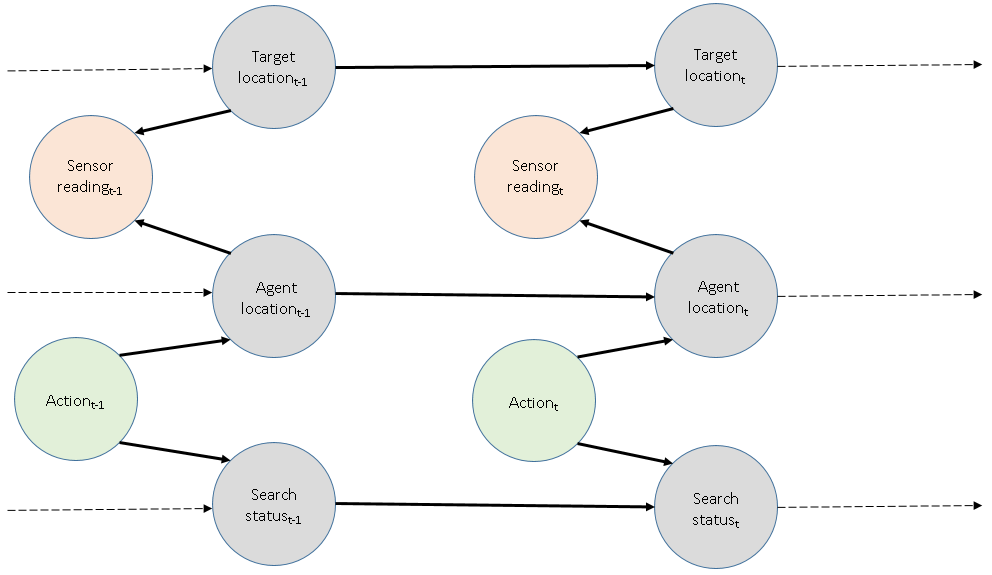
\includegraphics[width = 0.8\linewidth]{Chapters/MultiAgentTargetDetection/Figs/DBNWithMultipleHiddenState.PNG}
     \caption{First Version of the DBN representing the agent world model}
    \label{fig:FirstDBNUsed}
\end{figure}
A number of conditional probabilities are specified here in order to describe the factored joint distribution of the world model fully. The full tables are omitted as they are sparse. For brevity, we use the abbreviation Loc for Location.



\begin{figure}[H]
\scriptsize
\begin{equation}\label{eqn:EvidenceVarsProbs}
    %\centering
    p(SensorReading_t | AgentLoc_{t-1}, EvidenceLoc_{t-1})  = 
    \begin{cases}
    \alpha \quad \text{ if } SensorReading_t=1 \text{ and } EvidenceLoc_t \neq AgentLoc_t
    \\
    1-\beta \quad \text{ if } SensorReading_t=1 \text{ and } EvidenceLoc_t = AgentLoc_t
    \\
    \beta \quad \text{ if } SensorReading_t=0 \text{ and } EvidenceLoc_t \neq AgentLoc_t
    \\
    1-\alpha \quad \text{ if } SensorReading_t=0 \text{ and } EvidenceLoc_t \neq AgentLoc_t
    \end{cases}
    %
\end{equation}
\caption{Conditional Probability Distribution for the $Evidence$ Variable}
\end{figure}


\begin{figure}[H]
\scriptsize
\begin{equation}\label{eqn:TargetLocProbs}
    p(TargetLoc_{t} | TargetLoc_{t-1}) =
    \begin{cases}
    1 \quad \text{ if } TargetLoc_{t}=TargetLoc_{t-1}
    %agent returns correct target Loc.} 
    \\
    0 \quad \text { otherwise. }
    \end{cases}
\end{equation}
\caption{Conditional Probability Distribution for the $TargetLocation$ Variable}
\end{figure}





\begin{figure}[H]
\scriptsize
%\begin{equation}\label{eqn:SearchStatus}
    \begin{gather}\label{eqn:SearchStatus}
        p(SearchStatus_t | SearchStatus_{t-1}, Action_{t-1}) = \\
        \begin{cases}
        1 \quad \text{ if } SearchStatus_t = terminated\_x_i \text{ and } SearchStatus_{t-1} = terminated\_x_i 
        \\
        1 \quad \text{ if } Action_t = terminate\_x_i \text{ and } SearchStatus_{t-1}=ongoing \text{ and } SearchStatus_{t} = terminated\_x_i
        \\
        1 \quad \text{ if } Action_t = move\_x_i \text{ and } SearchStatus_{t-1}=ongoing \text{ and } SearchStatus_t=ongoing
        %agent returns correct target location.} 
        \\
        0 \quad \text { otherwise. }
        \end{cases}
    \end{gather}
%\end{equation}
\caption{Conditional Probability Distribution for the $SearchStatus$ Variable}
\end{figure}





\begin{figure}[H]
\scriptsize
    \begin{equation}\label{eqn:AgentLocation}
        p(AgentLoc_t | AgentLoc_{t-1}, Action_{t}) = 
        \begin{cases}
        1 \quad \text{ if } Action_t = move\_x_i \text{ and } AgentLoc_t = x_i
        \\
        1 \quad \text{ if } Action_t = terminate\_x_i \text{ and } AgentLoc_t = AgentLoc_{t-1}
        \\
        0 \quad \text{otherwise}
        \end{cases}
    \end{equation}
\caption{Conditional Probability Distribution for the $AgentLocation$ Variable}
\end{figure}


\normalsize
The semantics of the equations listed above is given here: 
\begin{enumerate}
    \item Equation \ref{eqn:EvidenceVarsProbs} uses two parameters, $\alpha$ and $\beta$, to represent the probability of making a false positive and false negative sensor reading, respectively. These are assumed to have been calculated by using pre-calibrated values of the sensor. This model is very flexible and does not stipulate any restrictions on the sensor other than that it must return a reading indicating that the target is present or not.
    \item  Equation \ref{eqn:TargetLocProbs} simply states that the location of the target does not change, even though it is hidden. It would be very easy to modify this to allow for moving target detection in the case of a non-static target.
    \item Equate \ref{eqn:SearchStatus} is also states a number of intuitive notions. The first line states that once the agent terminates the search, it remains over. The second line states that if the agent requests an ongoing search to terminate, then it does so deterministically. The third line states that if the agent chooses to move in an ongoing search, then the search remains ongoing.
    \item Equation \ref{eqn:AgentLocation} simply outlines that the agent moves to new locations deteministically. It also indicates that should the agent choose to terminate the search, then the environment enters a terminal state, indicating that the search is over.
\end{enumerate}


Note that despite the fact that some hidden state variables cannot be observed directly, it is still possible to infer their value exactly based on their starting state. For example, the position of the agent is a deterministic function of its actions and previous position. These variables could have been treated as variables that are internal to the agent rather than part of the hidden world state and many authors omit such variables for the sake of clarity.
\note{need to outline why I have included them - mainly because evidence probability depends on agent location as well as source location}


\subsubsection{Estimated State}
\workinprogress
Since the agent operates in a partially observable environment, the agent's internal state representation of the environment needs to take into account the fact that the current environment state is not certain. For this reason, a probability distribution over possible environment states is used by the agent to internally represent the environment state. The internal agent state is described mathematically by 
\[p(x_t | e_{1:t}, u_{1:t})\]
, which is the distribution of possible world states given all evidence and control actions up to the current time step, where $x_t$, $e_t$ and $u_t$ follow the conventions of being the hidden state variables, the evidence variables and the control action variables. The agent updates this state using the world model specified in the preceding chapter, using the filtering algorithm explained in section \ref{subsection:InferenceHMMDBN} of Chapter \ref{chapter:Background}. There are a couple of noteworthy points:
\begin{itemize}
    \item A distribution that has a single sharp peak would indicate that the agent believes that the target is at a specific location with high confidence. This is clearly preferred to a flat, uniform distribution representing uncertainty in relation to where the target might be.
    \item The only true source of uncertainty in the world state is introduced by the sensor. Therefore, analysis of this state representation in relation to the sensor model should provide insight into how the system performs.
\end{itemize}
In order to update the estimated state of the agent, the below equations are used, which are described in subsection \ref{subsection:InferenceHMMDBN}. For brevity $x_t$ denotes the hidden state variables, $e_t$ denotes the evidence variable and $u_t$ denotes the control action taken by the agent. The equations only describe the estimated state update for move actions, since if the agent terminates the search a terminal state is deterministically entered. The $SearchStatus$ variable is omitted from the equations since it only effects the equations if the $Action$ variable is to terminate the search.
\footnotesize
\begin{figure}[H]
\scriptsize
%\begin{equation}\label{eqn:SearchStatus}
    \begin{gather}\label{eqn:SearchStatus}
        p(AgentLoc_t = x, TargetLoc_t = y | e_{1:t}, u_{1:t}) = \\
        \begin{cases}
            \eta \alpha p(AgentLoc_{t-1} = x, TargetLoc_t = y | e_{1:t-1}, u_{1:t-1}) \text{ if $e_t$ is a positive reading and $AgentLoc_t \neq TargetLoc_t$} \\
            \eta \beta p(X_{t-1}=x_t | e_{1:t-1}, u_{1:t-1}) \text{ if $e_t$ is a negative reading and $Agent_loc_t$ = $TargetLoc_t$} \\
            \eta (1-\alpha) p(X_{t-1}=x_t | e_{1:t-1}, u_{1:t-1}) \text{ if $e_t$ is a negative reading and $Agent_loc_t \neq TargetLoc_t$} \\
            \eta (1-\beta) p(X_{t-1}=x_t | e_{1:t-1}, u_{1:t-1}) \text{ if $e_t$ is a positive reading and $Agent_loc_t$ = $TargetLoc_t$} \\
        \end{cases}
%\eta O_{t} T^{T} f_{1:t-1} 
    \end{gather}
\end{figure}
\normalsize


\subsection{Action Selection Strategies}\label{subsubsec:ActionSelection}
At each discrete time step the agent may either choose to terminate the search or move to a new location to take a measurement reading. The agent may choose which of these actions to perform based on its location, the search status and its internal representation of the environment, which are outlined in the preceding section. First we discuss how move actions are chosen, if the agent decides that the search should not be terminated at the current time step. We began by implementing some of the recommended basic search strategies outlined in the related works by \citeauthor{Chung2007ASearch} \cite{Chung2007ASearch} and \citeauthor{Waharte2010SupportingUAVs} \cite{Waharte2010SupportingUAVs}. These search methods are devised in order to optimize the agent's performance measure, which is set out in Section \ref{sssection:PerfMeas}. The results of applying these strategies are discussed in Section \ref{sec:SimulationResults}.\par 
%\note{In the following, might be good to mention the motivation in relation to the performance measure}
\textbf{Random Search}
This method serves as a baseline against which similar strategies can be compared. The agent simply chooses the next grid location to explore randomly from all possible grid locations. The expected number of moves needed to take a reading at all possible grid cells is given by the solution to the \textit{coupon collectors problem} \cite{Erdos1961OnTheory}, $nH_n$, where $H_n$ is the $n_{th}$ harmonic number and $n$ is the total number of grid cells, which gives a good idea of the expected amount of time that will be taken to conclude the search.

\textbf{$\epsilon$-Greedy Search}
A simple greedy search was implemented next, where the agent chooses to visit the grid cell with the highest estimated probability of containing the target in a localized region around the agent:
\footnotesize
\[
Action_t = \argmax_{NewLoc \in N(AgentLoc)}{p(TargetLoc = NewLoc, SearchStatus, AgentLocation| e_{1:t}, u_{1:t})}
\]
\normalsize
$N(AgentLoc)$ is a function that returns a neighborhood of locations around the agent's location and can be calibrated to trade off the cost of saccading between grid cells that may be far from each other against the cost of limiting the agents range to a narrow and possibly "cold" region.This method is designed bearing in mind that there may be motivation to explore some areas before others based on prior knowledge. 

%\textbf{$\epsilon$-greedy Search} Greedy search  simplest method to implement was an $\epsilon$-greedy action selection method, whereby the agent moves to the grid cell with the highest estimated probability in a pre-defined radius with probability 1-$\epsilon$ and a random grid cell in the pre-defined with probability $\epsilon$. This encourages the agent to exploit it's current know\par

\textbf{Saccadic Search}
This was proposed in \cite{Chung2007ASearch} and is a special case of $\epsilon$-greedy search. The idea is to mimic the behaviour of the human eye when looking at an image, whereby it "\textit{saccades}" from one salient feature to another. The consequence is that the most promising cells are explored at each time step, which means that the agent can be drawn to travel large distances in order to explore a peak in the spatial distribution given by the occupancy grid. Further details are given in \cite{Chung2007ASearch}.

\textbf{Sweep Search}
This strategy sweeps the region of interest systematically, aiming to take a reading at each grid cell an equal number of times while minimizing the total distance travelled. It then traverses this same path again in reverse order. This requires planning a trajectory in advance, which is often referred to in related literature as the \textit{complete coverage path}. Since the region to be swept is assumed to be a grid, where adjacent points are assumed to be equidistant, a number of heuristic solutions were available for use from Section \ref{sec:SceneSurveying}.\par

%\textbf{POMDP Based Search} 
%\note{Not sure if I should go into this at all. Work was done in understanding POMDPs and clearly the solution can be easily framed as a POMDP but my work stopped short in actually finding a solution to POMDP that works well}
%As outlined in 
%details. \par


\subsection{Search Termination}\label{subsubsec:SeachTerminationMethodology}

At each discrete timestep, the agent can either choose to move to a new grid location to record a sensor measurement or it can decide to terminate the search based on its estimated state of the environment. There is a trade-off in terminating the search early, which means that less time and resources are spent on continuing the search, versus the possibility of drawing misinformed conclusions from the search due to a lack of information. For example, if the agent receives a series of false positive readings at a given location, it could mistakenly choose to conclude that the target is present at a given location rather than sample further to gain confidence that it has correctly found the location of the target. Following this line of thinking, it is clear that a strategy needs to be devised to minimize the probability of drawing false conclusions, which is described in the performance measure set out in Section \ref{sssection:PerfMeas}.\par
\citeauthor{Pollock1971SearchInterfaces} outlines three commonly used criteria that can be used to make a decision whether to terminate the search or not: the \textit{Bayes Criterion}, which minimizes the expected cost per decision, the \textit{Minimax Criterion}, which chooses a decision which minimises the maximum expected cost and the \textit{Neyman-Pearson Criterion}, which uses a likelihood ratio test to determine the optimal decision to make \cite{Pollock1971SearchInterfaces}. These tests are proposed in the context of a target that is definitely present in the search region, but can be extended to incorporate the decision problem where the target may or may not be present. In addition, related work by \citeauthor{Chung2007ASearch} has addressed this problem using methods that use heuristics to make a decision whether to terminate the search or not \cite{Chung2007ASearch}. 

We ultimately choose to implement the Sequential Probability Ratio Test (SPRT), which is a hypothesis-testing framework developed by \citeauthor{Wald1950BayesProblems} to optimally deal with sequential decision problems, as opposed to traditional frameworks which assume that all the necessary data has been gathered prior to analysis \cite{Wald1950BayesProblems}. The background knowledge behind the SPRT can be found in Section \ref{subsec:SPRT}. An algorithm is also provided on how to perform this test in practice.
%The details of the proof of optimality of the SPRT is given in \cite{Wald1950BayesProblems} and we have outlined the details of how to perform hypothesis-testing using this framework in section <refer to the section>, along with the practical advantages and drawbacks of using it. 
We applied the SPRT algorithm to our problem to provide a search termination criteria using the following quantities: 
%In order to allow the agent to make a decision on whether to terminate the search or not, the following procedure was used: \note{Might be worthwhile simply outlining the algorithm}

\begin{gather}\label{eqn:SPRTQuantities}
H_0 : \text{The null hypothesis, the target is not present in the search region}\nonumber
\\ \nonumber
H_1 : \text{The alternative hypothesis, the target is present in the search region}\nonumber
\\ \nonumber
\alpha : \text{The maximum probability of making a type } \Romannum{1} \text{ error.} \nonumber
\\ \nonumber
\beta : \text{The maximum probability of making a type } \Romannum{2} \text{ error.}\nonumber
\\ \nonumber
\\ \nonumber
p_{0t} : \text{ The probability of observing the data $(e_1, ..., e_t)$ under the assumption of $H_0$} \nonumber
\\ \nonumber
p_{0t}=\sum_{loc=1}^{n} p(TargetLoc_t = loc, AgentLoc_t, SearchStatus_t| e_{1:t}, u_{1:t})\nonumber
\\ \nonumber
\\ \nonumber
p_{1t} : \text{ The likelihood of observing the data $(e_1, ..., e_t)$ under the assumption of $H_1$} \nonumber
\\ \nonumber
p_{1t}=p(TargetLoc_t = n+1, AgentLoc_t, SearchStatus_t | e_{1:t}, u_{1:t})\nonumber 
\end{gather}

$p_{0t}$ and $p_{1t}$ are calculated by using the evidence likelihood algorithm, which is described in detail in Section \ref{subsubsec:EvLikelihood}. The SPRT algorithm was then used at each timestep to decide whether to 
\begin{enumerate}
    \item Terminate the search accepting $H_0$, that the target is not present in the search region.
    \item Terminate the search accepting $H_1$, that the target is present in the search region. In this case, the target location with the highest estimated probability is returned as the target location.
    \item Continue the search, using the Action Selection Strategy described in Section \ref{subsubsec:ActionSelection}.
\end{enumerate}
In practice, we often took logarithmic transforms of the values used in the SPRT, to simplify some calculations and to be able to look at plots that are less heavily skewed and simpler to interpret.

\subsection{Analysis of Search Termination Criteria}
The two parameters, $\alpha$ and $\beta$ that the user needs to specify to perform the SPRT need to be chosen carefully and depend on the context of the search. As in the standard hypothesis testing context, it is important to consider the significance level and power of the test to ensure that they reflect the severity of drawing an incorrect conclusion \cite{IntroductionToMathematicalStatistics}. They can also help to perform analysis on how well the agent could perform, since setting a high threshold means that the agent may have to take a minimum number of samples at the correct target location in order to choose $H_0$ or $H_1$. \par

Figure \ref{fig:SPRTCutoffFunctionOfAlphaAndBeta} shows how A and B vary as functions of the parameters $\alpha$ and $\beta$ on a log scale
%\footnote{Tables of the values of A and B for varying for varying Type \Romannum{1} rates ($\alpha$) and Type \Romannum{2} ($\beta$) error rates may be referred to in Appendix \ref{chap:AppendixOne}.}. 
Tables of the values of A and B for varying for varying Type \Romannum{1} rates ($\alpha$) and Type \Romannum{2} ($\beta$) error rates may be referred to in Appendix \ref{chap:AppendixOne}.
If the log-likelihood ratio of the data lies in between the red and blue surfaces on the graph, another sample is taken. A projection of this plot is shown in Figure \ref{fig:VaryingSPRTParametersProjected1}:
\begin{enumerate}[label=(\alph*)]
    \item shows a plot of how varying the Type \Romannum{1} error rate $\alpha$ for a fixed Type \Romannum {2} error rate $\beta = 0.07$ affects the decision boundaries defined by A and B.
    \item shows a plot of how varying the Type \Romannum{2} error rate $\beta$ for a fixed Type \Romannum{1} error rate $\alpha = 0.1$ affects the decision boundaries defined by A and B.
\end{enumerate}

Figures \ref{fig:SPRTCutoffFunctionOfAlphaAndBeta} and \ref{fig:VaryingSPRTParametersProjected1} reflect the intuition behind the decision boundaries. The lower the probability of making either a Type \Romannum{1} or Type \Romannum{2} error, the further apart the decision boundary becomes, meaning the likelihood ratio must be very far apart from 1, which appears as 0 on the log scale. A likelihood ratio of 1 indicates maximum uncertainty. It is also possible to see that the surfaces meet when $\alpha=0.5$, $\beta=0.5$, which reflects the fact that immediately terminating the search will give a 0.5 probability of returning a false positive or false negative. \par

\note{Might be better off editing these images with explicit labels showing regions in which H0 and H1 will be accepted.}
Figure \ref{fig:VaryingSPRTParametersProjected2} shows the regions in which the SPRT will elect to take another sample (the green shaded region), to accept $H_0$, the upper red shaded region, and to accept $H_1$, the lower red shaded region. The blue line shows the log-likelihood ratio of $\frac{(e_{1:t} | H_0)}{p(e_{1:t} | H_1)}$ as a function of the agent belief that the target is present in the search region. 
\note{This is not really clear, should exaggerate this more}
Note that since the values of $\alpha$ and $\beta$ are significantly smaller in Figure \ref{fig:VaryingSPRTParametersProjected2} (b) than in Figure \ref{fig:VaryingSPRTParametersProjected2} (a), the acceptance region for $H_0$ and $H_1$ are significantly smaller in (b) than in (a).

\par
%varying the type \Romannum{1} error rate for a fixed type \Romannum{2} error rate affects the upper and lower threshold for cutting off the search. Figure \ref{fig:SPRTVaryingT2} shows how the varying the type \Romannum{2} error rate for a fixed type \Romannum{1} error rate affects the upper and lower threshold for cutting off the search. Note that as the varying error rate increases on the x-axis, the decision boundaries come closer together, reflecting the intuition that we are more willing to accept a mistaken conclusion.
%\begin{figure}
%    \centering
%    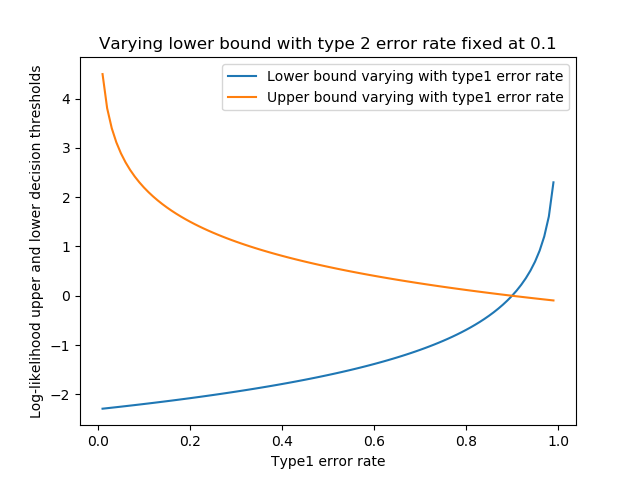
\includegraphics[width = 0.75\linewidth]{Chapters/MultiAgentTargetDetection/Figs/SearchTermination/SPRTDecisionThresholdVaryingT1ErrorRate.png}
%    \caption{The Log-likelihood upper and lower threshold for a varying type \Romannum{1} error rate and fixed type \Romannum{2} error rate.}
%    \label{fig:SPRTVaryingT1}
%\end{figure}

%\begin{figure}
%    \centering
%    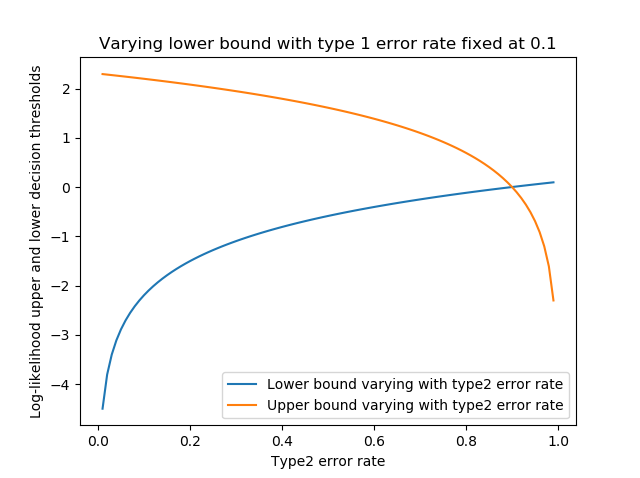
\includegraphics[width = 0.75\linewidth]{Chapters/MultiAgentTargetDetection/Figs/SearchTermination/SPRTDecisionThresholdVaryingT2ErrorRate.png}
%    \caption{The Log-likelihood upper and lower threshold for a varying type \Romannum{2} error rate and fixed type \Romannum{1} error rate.}
%    \label{fig:SPRTVaryingT2}
%\end{figure}

%Show how A and B vary for a fixed T1 or T2 error rate.
\begin{figure}[H]
    \centering
    \subfloat[Varying T\Romannum{1} error rate for a fixed T\Romannum{2} error rate]{{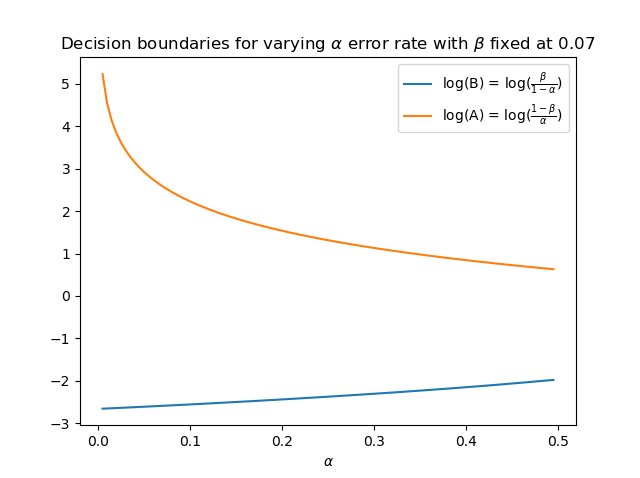
\includegraphics[width=11cm]{Chapters/MultiAgentTargetDetection/Figs/SearchTermination/AAndBVaryingWithAlpha.png} }}%
    \qquad
    \subfloat[Varying T\Romannum{2} error rate and fixed T\Romannum{1} error rate]{{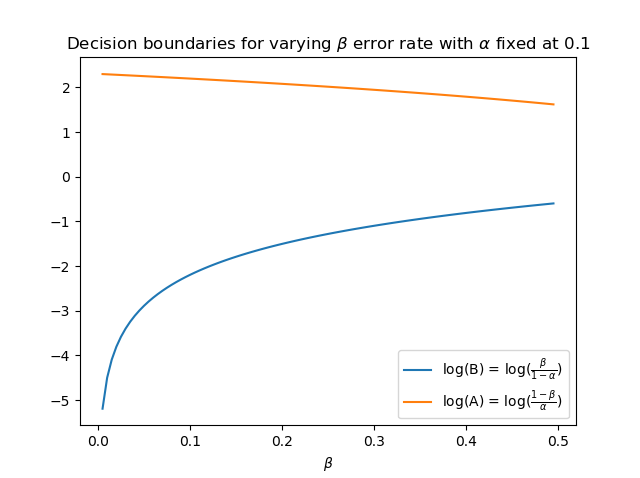
\includegraphics[width=11cm]{Chapters/MultiAgentTargetDetection/Figs/SearchTermination/AAndBVaryingWithBeta.png} }}%
    \caption{Upper and lower values of A and B for varying error rates. Values are shown on a log scale}%
    \label{fig:VaryingSPRTParametersProjected1}%
\end{figure}


%3-Dimensional plot to show how A and B vary with alpha and beta
\begin{figure}[h]
    \centering
    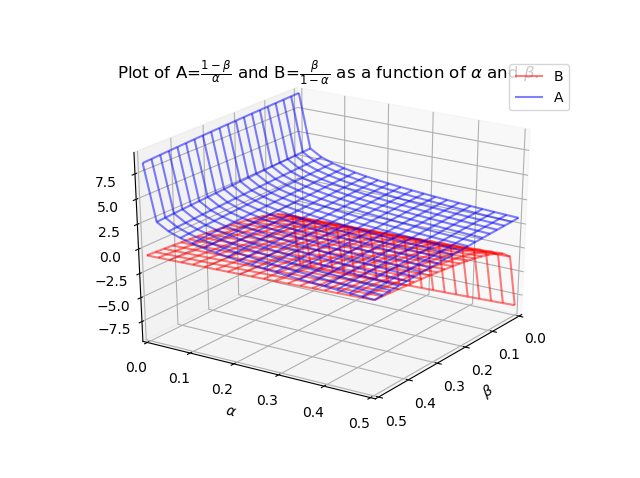
\includegraphics[width = 0.78\linewidth]{Chapters/MultiAgentTargetDetection/Figs/SearchTermination/AandBAsFunctionOfAlphaAndBetaLogTransform.png}
    \caption{The upper and lower SPRT bounds for acceptance and rejection of $H_0$, as functions of the significance and power of the test. Values are shown on a log scale.}
    \label{fig:SPRTCutoffFunctionOfAlphaAndBeta}
\end{figure}


%\begin{figure}
%    \centering
%    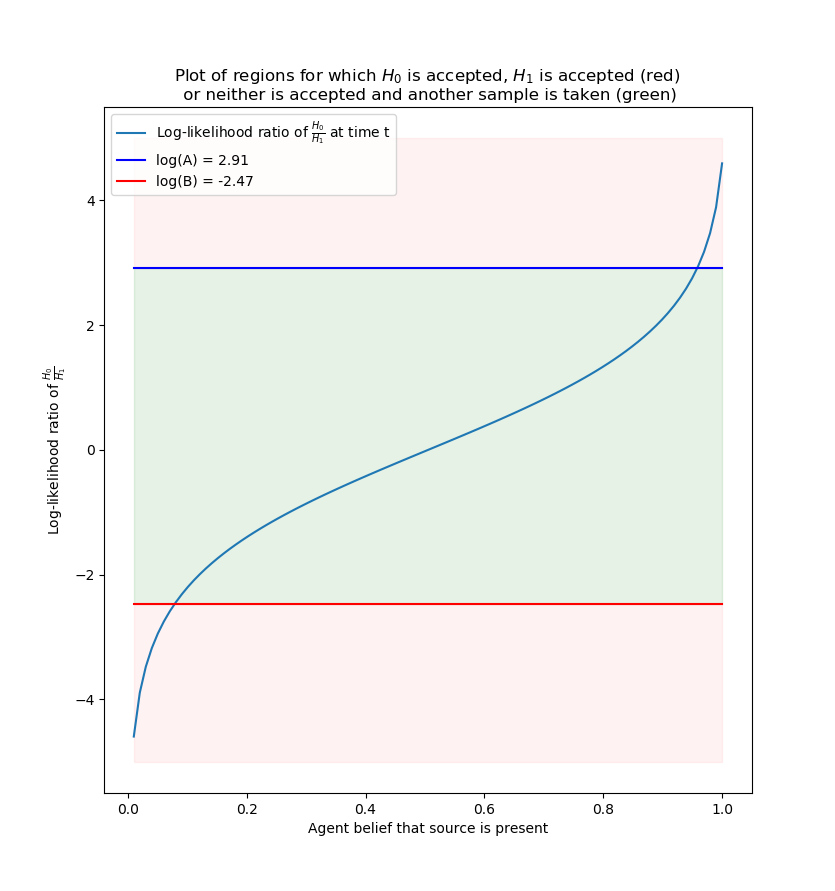
\includegraphics[width = 0.75\linewidth]{Chapters/MultiAgentTargetDetection/Figs/SearchTermination/CutoffRegions.png}
%    \caption{The cut-off regions of the SPRT for $\alpha=0.05$, $\beta=0.08$ as a function of agent belief in whether target is present or not. Values are shown on a log scale.}
%    \label{fig:SPRTLogLikelihoodRatio}
%\end{figure}

%showing how A and B create upper and lower limits for terminating the search
\begin{figure}[H]%
    \centering
    \subfloat[SPRT cut-off regions for $\alpha=0.05$, $\beta=0.08$]{{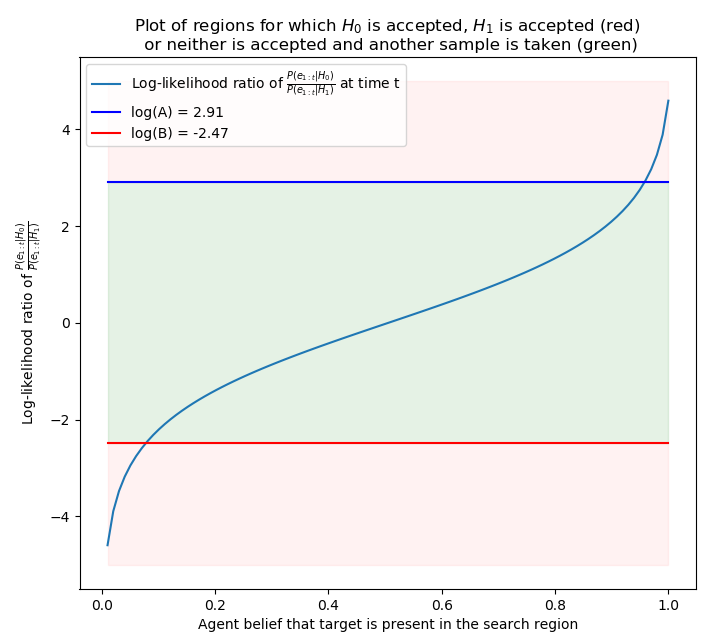
\includegraphics[width=11.5cm]{Chapters/MultiAgentTargetDetection/Figs/SearchTermination/CutoffRegionsAlphaPointZeroFiveBetaPointZeroEight.png} }}%
    \caption{} \label{fig:SPRTProjected1}
    %\qquad
\end{figure}
\begin{figure}[H]\ContinuedFloat
    \centering
    \subfloat[SPRT cut-off regions for $\alpha=0.01$, $\beta=0.02$ \label{fig:SPRTProjected2}]{{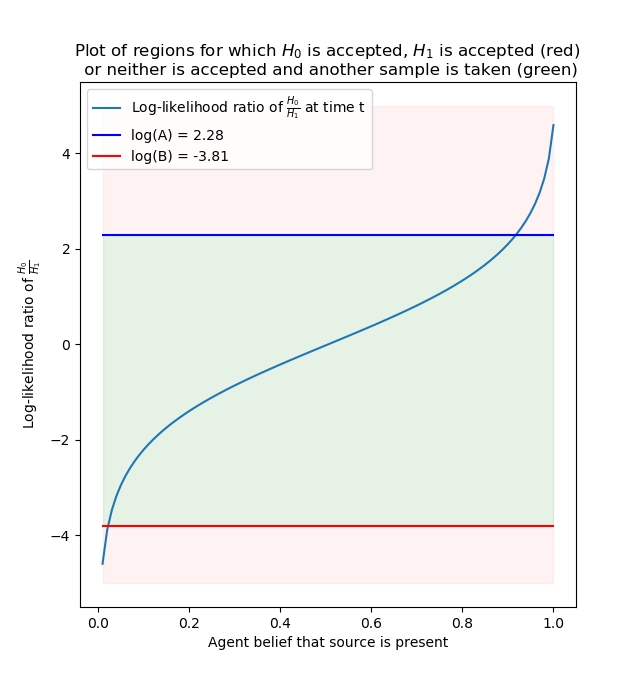
\includegraphics[width=11.5cm]{Chapters/MultiAgentTargetDetection/Figs/SearchTermination/CutoffRegionsAlphaPointOneBetaPointZeroTwo.png} }}%
    \caption{The cut-off regions of the SPRT for (a) $\alpha=0.05$, $\beta=0.08$ and (b) $\alpha=0.01$, $\beta=0.02$ as a function of agent belief in whether target is present or not. Values are shown on a log scale.}%
    \label{fig:VaryingSPRTParametersProjected2}%
\end{figure}



\note{maybe move tables to appendix}












